\documentclass{article}
\usepackage{iclr2027_conference,times}
\input{math_commands.tex}
\usepackage{hyperref}
\usepackage{url}
\usepackage{booktabs}
\usepackage{multirow}
\usepackage{amsmath,amssymb}
\usepackage{graphicx}
\usepackage{xcolor}
\usepackage{algorithm}
\usepackage{algorithmic}
\usepackage{tikz}
\usetikzlibrary{arrows.meta,positioning,shapes.geometric,calc,fit,backgrounds}
\usepackage{pgfplots}
\pgfplotsset{compat=1.18}
\usepackage{microtype}

% Colours used consistently in the architecture figure.
\definecolor{frozen}{RGB}{90,90,90}
\definecolor{trained}{RGB}{180,83,9}
\definecolor{trainedfill}{RGB}{253,240,224}
\definecolor{slowfill}{RGB}{243,243,243}

\newcommand{\fast}{\mathrm{fast}}
\newcommand{\slow}{\mathrm{slow}}
\newcommand{\gain}{g}
\newcommand{\method}{LitJev-S2}

\title{Thinking Fast and Slow:\\A Hybrid Thinking Model with Self-Routing}

% Submissions are anonymous. Uncomment \iclrfinalcopy for the camera-ready version.
\author{Anonymous authors\\
Paper under double-blind review}
%\iclrfinalcopy

\begin{document}

\maketitle

\begin{abstract}
System One decision models answer typed questions (a choice among options, a score on a scale, a yes/no) in a single forward pass by reading option logits at an answer boundary instead of generating text. They are fast and cheap, but they cannot reason, and on hard questions they are wrong. We ask whether such a model can decide, at no extra token cost, which questions are worth the price of slow thinking. We attach a small \emph{decision head} beside the language-model head at the readout position of a frozen backbone. The head reads the same hidden state that produces the fast answer and predicts the joint outcome of the fast path and of the backbone's own thinking mode: whether each would be right or wrong. A question is escalated when the predicted accuracy gain from thinking exceeds a cost $\lambda$ chosen at request time. Labels for the head are produced automatically by running both paths once on a labelled set; no human annotation of ``should think'' is needed, and no backbone weight is modified. On MMLU-Pro with a 4B-parameter Qwen backbone, fast-only accuracy is 0.540 and always-thinking accuracy is 0.740 at a mean cost of 994 generated tokens per question. Routing with the decision head reaches 0.717 while thinking on 53\% of questions, recovering 89\% of the accuracy gain for 53\% of the token cost, and beats a router that sees only the fast answer distribution at every escalation rate. The routing signal is carried by an intermediate layer's hidden state passed through a whitened low-rank projection; raw hidden states overfit at this data size.
\end{abstract}

\section{Introduction}

A growing class of deployed language-model workloads are not conversations but decisions: route this ticket, is this claim supported, how urgent is this state, which of these five actions next. Typed decision models such as Jev \citep{typesafe2026jev} serve exactly this shape. The caller supplies a state and a set of typed questions; the model returns, for each question, an option key, a probability distribution over the options, and a confidence, without generating a single answer token. The mechanism is old \citep{hendrycks2017baseline}: prefill the state, append each question and its options, and read the logits of the option codes at an answer boundary. What is new is treating this readout as the product, with a request/response contract that code can consume directly, and the resulting latency and cost, one to two orders of magnitude below generate-then-parse.

The price of the single pass is that the model cannot think. On questions that require multi-step reasoning the fast readout is a guess, and on MMLU-Pro \citep{wang2024mmlupro} a 4B backbone's fast readout is right 54\% of the time while the same backbone with its thinking mode enabled is right 74\% of the time. Always thinking closes the gap but costs a thousand generated tokens per question, which is the cost the fast path exists to avoid. The interesting regime is in between: think only where thinking pays. This is the division of labour that \citet{kahneman2011thinking} describes between a fast, automatic System~1 and a slow, deliberate System~2, with the added requirement that the hand-off be decided by the system itself.

This paper asks whether the model can make that call itself, in the same forward pass that produces the fast answer, without modifying the backbone. Our answer is a \emph{decision head} (Figure~\ref{fig:arch}): a small multilayer perceptron attached beside \texttt{lm\_head} at the readout position. It consumes the hidden state that the language-model head already reads, plus a few statistics of the fast answer distribution, and predicts a four-way outcome: whether the fast answer is right and whether the slow answer would be right. Escalation follows from a one-line rule, escalate when $P(\fast\ \text{wrong},\ \slow\ \text{right}) - P(\fast\ \text{right},\ \slow\ \text{wrong}) > \lambda$. The threshold $\lambda$ is the per-question price of thinking and is set at request time, so a deployment moves along the cost--accuracy curve without retraining.

Three properties make this practical. First, \textbf{the backbone is frozen and its behaviour is unchanged.} The fast path is exactly the original decision model; the slow path is exactly the backbone's native thinking mode; the head only decides which one answers. Second, \textbf{labels are free.} Because the slow path is deterministic given the frozen backbone, running both paths once on a labelled question set yields the four-way outcome label for every question. Third, \textbf{the decision costs no tokens.} The head reads a hidden state that is computed anyway.

We evaluate on MMLU-Pro with Qwen3.5-4B, holding out entire subject categories so that reported numbers measure transfer to unseen domains. Our contributions are:
\begin{itemize}
  \item A frozen-backbone architecture for self-routed fast/slow typed decisions, with a request-time cost knob and an unchanged fast-path contract (Section~\ref{sec:method}).
  \item A self-labelling procedure and a training recipe, grouped cross-validation over subject categories with a whitened low-rank bottleneck on the hidden state, that avoids the overfitting we observed with raw hidden states (Section~\ref{sec:training}).
  \item Evidence that the routing signal lives in an intermediate layer's hidden state and is not recoverable from the fast answer distribution alone: at matched escalation rates the head beats a distribution-only router by about three accuracy points, and recovers 89\% of the always-think gain at 53\% of its cost (Section~\ref{sec:experiments}).
\end{itemize}

We also report what did not work, including a prompt-template interaction that silently disabled thinking, because these failure modes are likely to recur for anyone building on hybrid-thinking checkpoints.

\section{Related work}

\paragraph{Typed decision models and constrained readout.}
Reading a classifier off a language model's next-token distribution over a small label set is the standard zero-shot protocol for multiple-choice evaluation \citep{hendrycks2021mmlu,wang2024mmlupro}. Jev \citep{typesafe2026jev} productised this readout as a typed decision API with parallel isolated questions and zero generated output tokens; a wave of open reproductions followed, including prefix-cached implementations on stock checkpoints \citep{ekzhang2026openjevsglang,zhihz2026openjev} and small trained scorers \citep{mapika2026decider}. Our fast path is one such reproduction. None of these systems can think; we add the ability to decide when to.

\paragraph{Adaptive computation and thinking budgets.}
Adaptive computation time \citep{graves2016act} and confident early exit \citep{schuster2022calm} allocate depth per token. Test-time scaling work \citep{snell2024scaling,muennighoff2025s1} shows that thinking length is a first-class compute knob, and AdaptThink \citep{zhang2025adaptthink} and L1 \citep{aggarwal2025l1} train the backbone with reinforcement learning to choose or bound its own reasoning length. We differ in leaving the backbone untouched: the routing policy is an external probe, trained by supervised learning on automatically produced labels, and the backbone's fast and slow behaviours are exactly what it shipped with.

\paragraph{Model routing.}
FrugalGPT \citep{chen2023frugalgpt} and RouteLLM \citep{ong2024routellm} route queries between cheap and expensive \emph{models} using a learned router over the query text. We route between two \emph{modes of the same model}, and the router reads the model's own internal state rather than the input, which is what allows it to cost nothing at inference: the state is already computed.

\paragraph{Confidence estimation from hidden states.}
Maximum softmax probability is a strong baseline for detecting misclassification \citep{hendrycks2017baseline}, and selective classification formalises the coverage--accuracy trade-off we plot \citep{geifman2017selective}. Language models carry information about their own correctness in their activations \citep{kadavath2022know,azaria2023internal}, recoverable with linear probes \citep{alain2017probes}. We use the same observation for a different target: not ``is this answer right'' but ``would thinking make it right''. Calibration in the sense of \citet{guo2017calibration} is a by-product: the head's $P(\fast\ \text{right})$ replaces the uncalibrated concentration statistic that the fast path would otherwise report.

\section{Method}
\label{sec:method}

\subsection{Fast path: shared prefill and branched readout}
\label{sec:fast}

A request carries a \emph{state} $s$ (text, or text plus an image) and $N$ typed questions $q_1,\dots,q_N$. Each question has a type in $\{\texttt{choice},\texttt{score},\texttt{noul}\}$ and a candidate set: the option keys for \texttt{choice}, the ordered levels for \texttt{score}, and $\{\text{false},\text{true}\}$ for \texttt{noul}. Following the typed-decision contract, question identifiers never enter the prompt and questions are isolated from one another.

The fast path uses two forward calls. The first prefills the state and a generic instruction once, producing a cache of key/value and, for hybrid backbones, recurrent states. The cache is replicated $N$ ways. The second call batches the $N$ question suffixes, each ending in the boundary string \texttt{Answer:}, against their cache copies. Candidate options are mapped at the boundary to single-token letter codes (\texttt{A}\dots\texttt{Z}, then \texttt{AA}\dots), verified per tokenizer, so that every candidate is exactly one token. At the boundary position $t_i$ of branch $i$ the model produces a final-layer hidden state $\vh_i\in\mathbb{R}^d$ and, through \texttt{lm\_head}, logits over the vocabulary. We slice the $K_i$ candidate logits $\vz_i\in\mathbb{R}^{K_i}$ and set $\vp_i=\mathrm{softmax}(\vz_i/\tau)$. The typed answer is assembled in code: the argmax key for \texttt{choice}, the probability-weighted level index for \texttt{score}, and $p(\text{true})$ for \texttt{noul}. No token is generated.

\subsection{Decision head}
\label{sec:head}

We attach a second reader at the same position (Figure~\ref{fig:arch}). Its input is the concatenation of (i) the hidden state $\vh_i^{(\ell)}$ at the boundary position from one chosen layer $\ell$, which need not be the final layer, and (ii) an eight-dimensional statistic vector $\vs_i$ of the fast distribution: maximum probability, normalised entropy, top-two margin, normalised Gini concentration, $\log K_i$, and a one-hot question type. The statistics are scale-free, so the head transfers across candidate-set sizes.

The head standardises its input with training-set moments, projects the hidden block through a whitened PCA basis $\mW\in\mathbb{R}^{d\times r}$ with $r\ll d$ (Section~\ref{sec:training}), and applies a two-layer MLP:
\begin{equation}
  \vu_i = \big[\,\mW^\top \tilde{\vh}_i^{(\ell)};\ \tilde{\vs}_i\,\big],\qquad
  \vo_i = \mathrm{softmax}\big(\mW_2\,\mathrm{GELU}(\mW_1\vu_i+\vb_1)+\vb_2\big)\in\Delta^{4},
\end{equation}
where tildes denote standardised quantities. The four outputs are the joint outcome probabilities
\begin{equation}
  \vo_i=\big(P(\fast\checkmark,\slow\checkmark),\ P(\fast\checkmark,\slow\times),\ P(\fast\times,\slow\checkmark),\ P(\fast\times,\slow\times)\big).
\end{equation}
Two quantities are derived. The \emph{confidence} reported to the caller is $c_i=\vo_{i,1}+\vo_{i,2}=P(\fast\checkmark)$, a probability of correctness rather than a shape statistic of the distribution. The \emph{escalation gain} is
\begin{equation}
  \gain_i=\vo_{i,3}-\vo_{i,2}=P(\fast\times,\slow\checkmark)-P(\fast\checkmark,\slow\times),
  \label{eq:gain}
\end{equation}
the expected change in accuracy from switching this question to the slow path. Predicting the joint outcome rather than fast correctness alone matters: a question the fast path gets wrong is not worth escalating if the slow path would also get it wrong, and a question the fast path gets right can be harmed by thinking (4.6\% of held-out questions in our data).

\begin{figure}[t]
\centering
% Architecture figure. Coordinates in mm; the drawing spans x = 1..137, inside the 139.7mm text width.
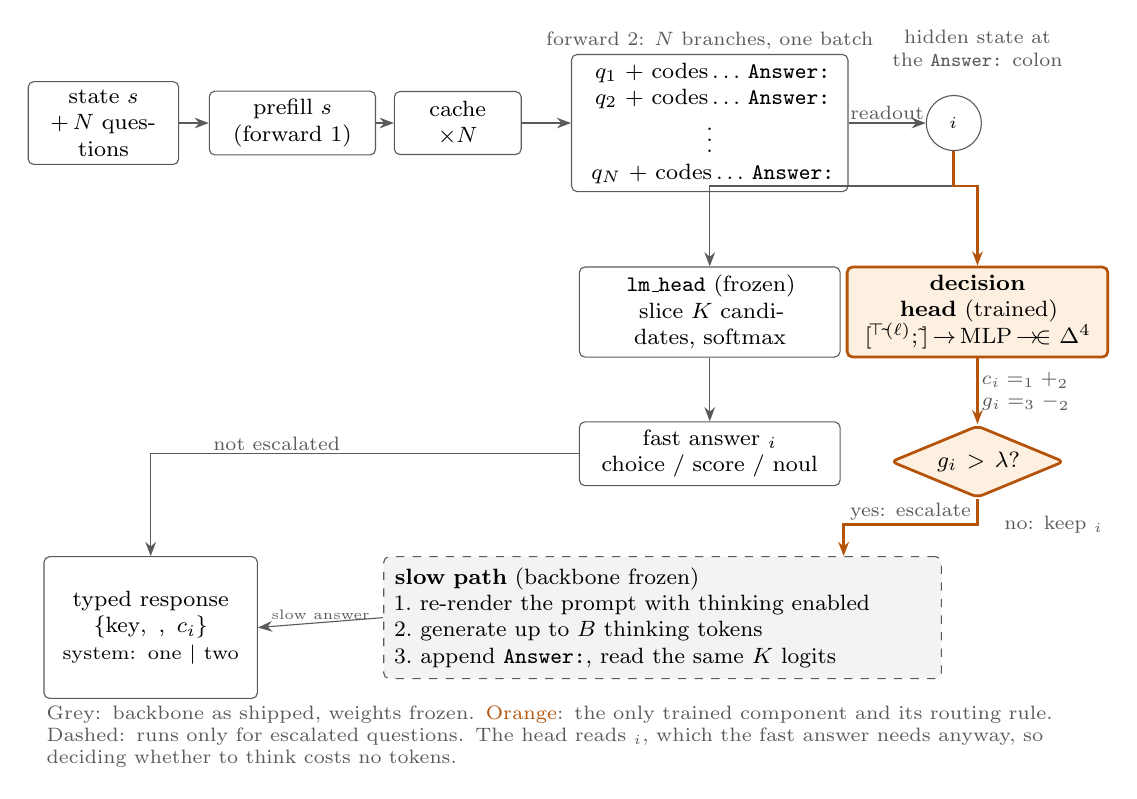
\begin{tikzpicture}[
  x=1mm, y=1mm, font=\footnotesize,
  box/.style={draw=frozen, rounded corners=2pt, minimum height=8mm, inner sep=3pt, align=center, text width=#1},
  tbox/.style={draw=trained, line width=1pt, fill=trainedfill, rounded corners=2pt, minimum height=8mm, inner sep=3pt, align=center, text width=#1},
  arr/.style={-{Stealth[length=1.8mm]}, draw=frozen},
  tarr/.style={-{Stealth[length=1.8mm]}, draw=trained, line width=1pt},
  lab/.style={font=\scriptsize, text=frozen, inner sep=1pt},
]
% ---- row 1: fast path
\node[box=17mm] (req) at (10,0) {state $s$\\$+\,N$ questions};
\node[box=19mm] (pre) at (34,0) {prefill $s$\\(forward 1)};
\node[box=14mm] (cache) at (55,0) {cache\\$\times N$};
\node[box=33mm, minimum height=16mm] (br) at (87,0) {$q_1$ + codes\,\dots\,\texttt{Answer:}\\$q_2$ + codes\,\dots\,\texttt{Answer:}\\$\vdots$\\$q_N$ + codes\,\dots\,\texttt{Answer:}};
\node[circle, draw=frozen, minimum size=7mm, inner sep=0pt] (h) at (118,0) {$\vh_i$};
\draw[arr] (req) -- (pre);
\draw[arr] (pre) -- (cache);
\draw[arr] (cache) -- (br);
\node[lab] at (87,10.5) {forward 2: $N$ branches, one batch};
\draw[arr] (br) -- node[lab, above] {readout} (h);
\node[lab, align=center] at (121,9.5) {hidden state at\\the \texttt{Answer:} colon};

% ---- row 2: the two heads
\node[box=31mm] (lm) at (87,-24) {\texttt{lm\_head} (frozen)\\slice $K$ candidates, softmax};
\node[tbox=31mm] (dh) at (121,-24) {\textbf{decision head} (trained)\\$[\mW^{\!\top}\tilde\vh^{(\ell)};\tilde\vs]\!\to\!\text{MLP}\!\to\!\vo\in\Delta^4$};
\draw[arr] (h.south) -- (118,-8) -| (lm.north);
\draw[tarr] (h.south) -- (118,-8) -| (dh.north);

% ---- row 3: fast answer and gate
\node[box=31mm] (fa) at (87,-42) {fast answer $\vp_i$\\choice / score / noul};
\node[tbox=18mm, shape=diamond, aspect=2.4, inner sep=0pt, text width=16mm] (gate) at (121,-43) {$\gain_i>\lambda$?};
\draw[arr] (lm) -- (fa);
\draw[tarr] (dh) -- node[lab, right, align=left] {$c_i=\vo_1{+}\vo_2$\\$\gain_i=\vo_3{-}\vo_2$} (gate);

% ---- row 4: response and slow path (tops aligned at y = -55)
\node[box=25mm, minimum height=18mm, anchor=north] (resp) at (16,-55) {typed response\\$\{\text{key},\ \vp,\ c_i\}$\\{\scriptsize system: one $|$ two}};
\node[draw=frozen, dashed, fill=slowfill, rounded corners=2pt, align=left, text width=68mm, inner sep=4pt, anchor=north] (slow) at (81,-55)
  {\textbf{slow path} (backbone frozen)\\
   1.\ re-render the prompt with thinking enabled\\
   2.\ generate up to $B$ thinking tokens\\
   3.\ append \texttt{Answer:}, read the same $K$ logits};
\draw[tarr] (gate.south) -- (121,-51) -| node[lab, above, pos=0.25] {yes: escalate} (104,-51) -- (104,-55);
\node[lab, anchor=west] at (124,-51) {no: keep $\vp_i$};
\draw[arr] (fa.west) -- (56,-42) -| node[lab, above, pos=0.3] {not escalated} (resp.north);
\draw[arr] (slow.west) -- node[lab, above, font=\tiny] {slow answer} (resp.east);

% ---- legend, anchored below the lower row
\node[lab, align=left, text width=128mm, anchor=north west] at ($(resp.north west |- slow.south)+(0,-3)$)
  {Grey: backbone as shipped, weights frozen. \textcolor{trained}{Orange}: the only trained component and its routing rule. Dashed: runs only for escalated questions. The head reads $\vh_i$, which the fast answer needs anyway, so deciding whether to think costs no tokens.};
\end{tikzpicture}

\caption{\method{} on one request. The state is prefilled once; $N$ question branches share the cache and are read out in one batched forward. At the readout position the frozen \texttt{lm\_head} produces the fast answer while the decision head predicts the joint (fast, slow) outcome. Questions whose escalation gain exceeds the request-time cost $\lambda$ are re-run through the backbone's own thinking mode and read out again at the same boundary.}
\label{fig:arch}
\end{figure}

\subsection{Routing rule and cost model}
\label{sec:routing}

Let $a_i^{\fast},a_i^{\slow}\in\{0,1\}$ be the correctness of the two paths and $T_i$ the number of thinking tokens the slow path generates. Escalating question $i$ changes expected accuracy by $\gain_i$ and costs $T_i$ tokens. With a per-token price the optimal policy escalates when $\gain_i>\lambda$ for a $\lambda$ proportional to that price. We therefore expose $\lambda$ directly on the request:
\begin{equation}
  \text{escalate}_i=\mathbb{1}[\gain_i>\lambda].
\end{equation}
$\lambda=0$ escalates whenever thinking is expected to help at all; $\lambda>0$ demands a margin; $\lambda<0$ escalates even at a small expected loss and approaches always-thinking. Because $\lambda$ never enters training, a deployment sweeps the coverage--accuracy curve by changing one number. The routed accuracy at threshold $\lambda$ on a set $\mathcal{D}$ is
\begin{equation}
  \mathrm{Acc}(\lambda)=\frac{1}{|\mathcal{D}|}\sum_{i\in\mathcal{D}}\Big(\mathbb{1}[\gain_i>\lambda]\,a_i^{\slow}+\mathbb{1}[\gain_i\le\lambda]\,a_i^{\fast}\Big),
\end{equation}
and the expected generated tokens per question is $\frac{1}{|\mathcal{D}|}\sum_i\mathbb{1}[\gain_i>\lambda]\,T_i$. A random router that escalates a fraction $\rho$ of questions attains $\mathrm{Acc}=\bar a^{\fast}+\rho\,(\bar a^{\slow}-\bar a^{\fast})$, a straight line between the two endpoints; a useful router lies above it.

\subsection{Slow path}
\label{sec:slow}

Escalated questions are re-run with the backbone's thinking mode. Hybrid-thinking checkpoints such as Qwen3 \citep{yang2025qwen3} decide whether to reason from the chat template: with thinking disabled the template inserts an empty \texttt{<think>\textbackslash n\textbackslash n</think>} block before the assistant turn, and with thinking enabled it ends the prompt with an open \texttt{<think>}. The fast prefix is rendered with thinking disabled. Appending \texttt{<think>} to it does not work: the model has already seen a closed thinking block and closes the new one after a single token (Section~\ref{sec:lessons}). The slow path therefore renders its own prompt from scratch with thinking enabled, placing the question body in the user turn, generates greedily until \texttt{</think>} or a budget of $B$ tokens, then appends the same \texttt{Answer:} boundary and reads the same $K$ candidate logits. The typed answer is assembled exactly as on the fast path; nothing is parsed from generated text. Escalated questions are batched together for generation. The response reports \texttt{output\_tokens} equal to the thinking tokens used, and marks each answer with the system that produced it.

\subsection{Training the decision head}
\label{sec:training}

\paragraph{Self-labelling.}
The slow path is a deterministic function of the frozen backbone, so its correctness on a labelled question is a fixed attribute of that question. Given a set of questions with gold answers, we run the fast path (recording $\vh_i^{(\ell)}$ for a few candidate layers $\ell$ and the statistics $\vs_i$) and the slow path (recording $a_i^{\slow}$ and $T_i$), compare both with gold, and obtain the four-way label $y_i\in\{0,1,2,3\}$ (Algorithm~\ref{alg:collect}). Gold answers are compared locally after both passes and never enter a prompt. Nobody labels ``should this question be escalated''.

\begin{algorithm}[t]
\caption{Self-labelled data collection}
\label{alg:collect}
\begin{algorithmic}[1]
\REQUIRE frozen backbone $f$, labelled questions $\{(s_i,q_i,y^\star_i)\}$, candidate layers $L$, budget $B$
\FOR{each batch of ten questions with shared state $s$}
  \STATE $\{(\vz_i,\{\vh_i^{(\ell)}\}_{\ell\in L})\}\leftarrow\textsc{FastPath}(f,s,\{q_i\})$ \COMMENT{prefill once, one branched forward}
  \STATE $\{(\vz_i^{\slow},T_i)\}\leftarrow\textsc{SlowPath}(f,s,\{q_i\},B)$ \COMMENT{thinking on, same readout boundary}
  \FOR{each question $i$}
    \STATE $a_i^{\fast}\leftarrow\mathbb{1}[\arg\max\vz_i=y^\star_i]$,\quad $a_i^{\slow}\leftarrow\mathbb{1}[\arg\max\vz_i^{\slow}=y^\star_i]$
    \STATE $y_i\leftarrow 2\,(1-a_i^{\fast})+(1-a_i^{\slow})$ \COMMENT{$0$: both right, $1$: fast only, $2$: slow only, $3$: neither}
    \STATE $\vs_i\leftarrow\textsc{Stats}(\mathrm{softmax}(\vz_i),\ \mathrm{type}(q_i))$
    \STATE store $(\{\vh_i^{(\ell)}\},\vs_i,y_i,a_i^{\fast},a_i^{\slow},T_i,\mathrm{category}(q_i))$
  \ENDFOR
\ENDFOR
\end{algorithmic}
\end{algorithm}

\paragraph{Objective and regularisation.}
The head is trained by class-weighted cross-entropy on $y_i$ with AdamW \citep{loshchilov2019adamw}, weight decay $0.05$, dropout $0.3$, and early stopping on a validation slice of the training set. Two ingredients were necessary. First, the hidden state is high-dimensional ($d=2560$ for the 4B backbone) relative to the number of labelled questions (about a thousand), and an MLP on the raw standardised $\vh$ memorises the training set: in our first run training loss fell to $0.002$ while held-out routing quality dropped below a router that ignores $\vh$ entirely. We therefore fit a whitened PCA basis $\mW$ on the standardised training hidden states and feed the head only the top $r$ components. Second, the choice of layer and of $r$ must not see the test data. We hold out whole subject categories as the test set and select the feature configuration by $K$-fold cross-validation grouped by category on the remaining data, scoring each configuration by the routing AUROC: how well $\gain_i$ ranks the questions on which thinking helps ($y_i=2$) above the rest (Algorithm~\ref{alg:train}). Selection on a single validation split was unstable at this data size and chose configurations that did not transfer.

\begin{algorithm}[t]
\caption{Decision head training with grouped selection}
\label{alg:train}
\begin{algorithmic}[1]
\REQUIRE records from Algorithm~\ref{alg:collect}, held-out categories $\mathcal{C}_{\text{test}}$, folds $K$, candidate configurations $\Theta$ (layer $\ell$, rank $r$, width $w$)
\STATE split records into $\mathcal{D}_{\text{train}}$ and $\mathcal{D}_{\text{test}}$ by category
\STATE assign each training category to one of $K$ folds
\FOR{each configuration $\theta\in\Theta$}
  \FOR{$k=1,\dots,K$}
    \STATE fit standardiser and PCA basis $\mW_\theta$ on folds $\ne k$; train head $H_\theta^{(k)}$ on folds $\ne k$ with early stopping
    \STATE $\mathrm{score}_k\leftarrow\mathrm{AUROC}\big(\gain_i(H_\theta^{(k)}),\ \mathbb{1}[y_i=2]\big)$ over fold $k$
  \ENDFOR
  \STATE $\mathrm{score}_\theta\leftarrow\frac{1}{K}\sum_k\mathrm{score}_k$
\ENDFOR
\STATE $\theta^\star\leftarrow\arg\max_\theta\mathrm{score}_\theta$
\STATE fit $\mW_{\theta^\star}$ and train $H_{\theta^\star}$ on all of $\mathcal{D}_{\text{train}}$
\STATE report $\mathrm{Acc}(\lambda)$, escalation rate, and AUROCs of $H_{\theta^\star}$ on $\mathcal{D}_{\text{test}}$
\end{algorithmic}
\end{algorithm}

\paragraph{Candidates.}
$\Theta$ contains a \emph{stats-only} head (no hidden state; this is the floor that $\vh$ must beat to justify its cost), one raw-$\vh$ head per collected layer, and one PCA-bottleneck head per collected layer. The stats-only head is itself a useful artefact: it needs no hidden states at inference and can be served by any implementation of the fast path.

\paragraph{Serving.}
The trained head is a single safetensors file that records the backbone identifier and revision, the prompt format, the layer, and the PCA rank; the server refuses a head whose metadata does not match the loaded backbone. The standard endpoint is unchanged. A second endpoint accepts the same request body plus an optional $\{\lambda,B\}$ block and returns the same response shape.

\section{Experiments}
\label{sec:experiments}

\subsection{Setup}

\paragraph{Backbone.}
Qwen3.5-4B, a hybrid checkpoint interleaving Gated DeltaNet layers \citep{yang2024gateddelta} with full attention (32 layers, $d=2560$), served in bfloat16 through Hugging Face Transformers \citep{wolf2020transformers} on one H100. Cache replication copies both key/value and recurrent states. We chose a small backbone so that the fast/slow gap is large and the experiment is cheap; the question of whether the gap and the routing signal persist at larger scale is left open.

\paragraph{Data.}
MMLU-Pro \citep{wang2024mmlupro}, test split, 1{,}500 questions sampled with stride 8 across all 14 subject categories, each with up to ten options. Three categories (chemistry, economics, psychology; 346 questions) are held out entirely as the test set; the remaining eleven (1{,}154 questions) form the training set and the $K=4$ selection folds. Every question is a \texttt{choice} question. Ten questions share one request with a generic state, matching the deployed ten-question batch.

\paragraph{Slow path.}
Greedy decoding, thinking budget $B=1024$ tokens. The backbone hit the budget on 90.3\% of questions (mean 994 tokens), so slow-path accuracy here is a floor and the gap to the fast path an underestimate.

\paragraph{Head.}
Collected layers $\ell\in\{-1,16,24\}$ where $-1$ is the final normalised output. PCA rank $r=64$, hidden width $w=64$ for bottleneck heads and $256$ for raw heads, $32$ for the stats-only head. Probe training for selection runs 10 epochs; the final head 60 epochs with patience 6. All training is on CPU and takes under a minute per configuration.

\paragraph{Metrics.}
Accuracy on the held-out categories as a function of escalation rate, swept over $\lambda$; AUROC of $\gain_i$ for ranking questions where thinking helps (\emph{routing AUROC}); AUROC of the confidence $c_i$ for fast-answer correctness; and expected thinking tokens per question. Baselines: fast only, slow only, the random-routing line, and the stats-only head.

\subsection{Main result}

\begin{table}[t]
\caption{Held-out accuracy and cost on three unseen MMLU-Pro categories (346 questions), Qwen3.5-4B. Tokens are mean generated thinking tokens per question. ``Gain kept'' is the fraction of the fast$\to$slow accuracy gain recovered.}
\label{tab:main}
\centering
\small
\begin{tabular}{llrrrr}
\toprule
Policy & $\lambda$ & Escalation & Accuracy & Tokens/q & Gain kept \\
\midrule
Fast only (System One) & -- & 0\% & 0.540 & 0 & 0\% \\
Slow only (always think) & -- & 100\% & 0.740 & 994 & 100\% \\
\midrule
Random routing & -- & 53\% & 0.646 & 527 & 53\% \\
Stats-only head & 0 & 48\% & 0.682 & 477 & 71\% \\
\method{} (layer 24, PCA-64) & $0.1$ & 35\% & 0.691 & 345 & 76\% \\
\method{} (layer 24, PCA-64) & $0$ & 53\% & \textbf{0.717} & 526 & 89\% \\
\method{} (layer 24, PCA-64) & $-0.1$ & 84\% & 0.728 & 830 & 94\% \\
\bottomrule
\end{tabular}
\end{table}

Table~\ref{tab:main} and Figure~\ref{fig:curve} give the main result. Thinking helps on 24.6\% of held-out questions and hurts on 4.6\%, so the ceiling for any router is 0.740 and the fast floor is 0.540. At $\lambda=0$ the decision head escalates 53\% of questions and reaches 0.717: 89\% of the available gain for 53\% of the token cost. At $\lambda=0.1$ it keeps 76\% of the gain for 35\% of the cost. The curve lies above the random-routing line everywhere and above the stats-only head at every escalation rate, by about three accuracy points in the middle of the range (0.717 vs.\ 0.682 near 50\% escalation; 0.691 vs.\ 0.656 near 33\%).

\begin{figure}[t]
\centering
\begin{tikzpicture}
\begin{axis}[
  width=0.62\linewidth, height=0.42\linewidth,
  xlabel={escalation rate (fraction of questions sent to the slow path)},
  ylabel={held-out accuracy},
  xmin=0, xmax=1, ymin=0.52, ymax=0.76,
  grid=major, grid style={gray!25},
  legend pos=north west, legend style={font=\scriptsize},
  tick label style={font=\scriptsize}, label style={font=\small},
  every axis plot/.append style={line width=0.9pt},
]
\addplot[frozen, dashed, domain=0:1, samples=2] {0.5405 + x*(0.7399-0.5405)};
\addlegendentry{random routing}
\addplot[trained, mark=*, mark size=1.4pt] table[x=rate, y=acc] {curve_head.dat};
\addlegendentry{\method{} head (layer 24, PCA-64)}
\addplot[blue!60!black, mark=square*, mark size=1.3pt] table[x=rate, y=acc] {curve_stats.dat};
\addlegendentry{stats-only head}
\addplot[frozen, only marks, mark=diamond*, mark size=2.2pt] coordinates {(0,0.5405) (1,0.7399)};
\addlegendentry{fast only / slow only}
\addplot[trained, only marks, mark=o, mark size=3.2pt, line width=0.8pt] coordinates {(0.5289,0.7168)};
\addlegendentry{$\lambda=0$ operating point}
\end{axis}
\end{tikzpicture}
\caption{Coverage--accuracy curves on held-out categories. Each marker is one value of $\lambda$. The decision head dominates both the random-routing line and a router that sees only the fast answer distribution. No router at this AUROC reaches the slow-only point; the value is keeping most of the gain at a fraction of the cost.}
\label{fig:curve}
\end{figure}

\subsection{Where the routing signal lives}
\label{sec:features}

\begin{table}[t]
\caption{Feature configurations. \emph{CV} columns are means over the four category folds of the training set and drive selection; \emph{test} columns are on the held-out categories and are reported for all configurations only for analysis. Routing AUROC ranks questions where thinking helps; fast AUROC ranks fast-correct questions. The selected configuration is in bold. Non-parametric baselines on the test set: max probability 0.836, concentration 0.842 (fast AUROC).}
\label{tab:features}
\centering
\small
\begin{tabular}{lcccccc}
\toprule
& & \multicolumn{2}{c}{CV (selection)} & \multicolumn{2}{c}{Test (held-out)} \\
\cmidrule(lr){3-4}\cmidrule(lr){5-6}
Configuration & Input dim & Routing & Fast & Routing & Fast \\
\midrule
Stats only & 8 & 0.671 & 0.757 & 0.704 & 0.838 \\
Layer $-1$, raw & 2568 & 0.700 & 0.748 & 0.677 & 0.824 \\
Layer $-1$, PCA-64 & 72 & 0.694 & 0.753 & 0.648 & 0.843 \\
Layer 16, raw & 2568 & 0.701 & 0.666 & 0.644 & 0.738 \\
Layer 16, PCA-64 & 72 & 0.668 & 0.729 & 0.716 & 0.837 \\
Layer 24, raw & 2568 & 0.729 & 0.748 & 0.718 & 0.824 \\
\textbf{Layer 24, PCA-64} & 72 & \textbf{0.758} & 0.766 & \textbf{0.721} & 0.834 \\
\bottomrule
\end{tabular}
\end{table}

Table~\ref{tab:features} separates two questions. \emph{Does the hidden state add anything beyond the fast distribution?} Yes, for routing: the selected configuration's routing AUROC exceeds the stats-only head both in cross-validation (0.758 vs.\ 0.671) and on held-out categories (0.721 vs.\ 0.704), and this is what produces the three-point accuracy margin in Table~\ref{tab:main}. \emph{Does it add anything for confidence?} No: fast-correct AUROC is 0.83--0.84 for every configuration and for the parameter-free max-probability baseline. The fast distribution already knows when the fast answer is wrong; what it does not know is whether thinking would fix it, and that is what the hidden state contributes.

Two further observations. Layer 24 of 32 carries a stronger routing signal than the final normalised output, consistent with probing results that place self-knowledge in intermediate layers \citep{azaria2023internal}. And the PCA bottleneck is not optional at this data size: raw 2560-dimensional inputs score lower than their bottlenecked counterparts on the layer that matters and, in an earlier 1{,}000-question run, fell below the stats-only floor.

\subsection{Per-category behaviour}

Table~\ref{tab:categories} in the appendix breaks the full 1{,}500 questions down by subject. The fraction of questions where thinking helps ranges from 10\% (biology) to 50\% (math), and the fraction where it hurts from under 1\% (physics) to 9\% (engineering, where the slow path barely improves on the fast one). A good router must therefore be subject-sensitive, and the head sees no subject label; whatever it learns about subjects it learns from the hidden state. The held-out categories span this range (chemistry 35\% helps, psychology 13\%), so the reported numbers are not from an easy slice.

\subsection{Cost}

At $\lambda=0$ the routed policy generates 526 thinking tokens per question in expectation against 994 for always-thinking, and the decision itself is free: the head is a $72\to64\to4$ MLP evaluated on a vector the fast path already produces. The fast path's own cost is unchanged at two forward calls and zero generated tokens. At the current 90\% budget-hit rate the slow path is dominated by generation, so the token ratio is a faithful proxy for latency and GPU time.

\section{Lessons from failed runs}
\label{sec:lessons}

We report three failures because each is easy to reproduce and hard to diagnose from aggregate metrics.

\paragraph{The slow path that never thought.}
Our first implementation appended \texttt{<think>} to the fast prefix. The smoke test reported a thinking length of exactly one token on every question, and 1{,}000 questions were collected before the aggregate looked wrong. The cause is the empty thinking block that the chat template inserts when thinking is disabled: the model treats reasoning as already finished. The fix (Section~\ref{sec:slow}) is to render the slow prompt with thinking enabled. Any pipeline that shares a prefix between a non-thinking and a thinking mode of a hybrid checkpoint should assert on thinking length.

\paragraph{Truncated reasoning underestimates the slow path.}
With $B=512$, the backbone hit the budget on 98.5\% of questions and slow-only accuracy was 0.616; with $B=1024$ it is 0.740. In the 512 run the routed policy appeared to \emph{exceed} always-thinking (0.642 vs.\ 0.616), which is impossible for a router with imperfect knowledge and was an artefact of truncation: escalation was selecting the questions the truncated slow path could still finish. We regard 1024 as a floor too.

\paragraph{Overfitting and unstable selection.}
Raw hidden states with $\sim$750 training examples drove training loss to $0.002$ and held-out routing AUROC below the stats-only head; selecting the layer on a single validation split then chose a raw configuration that did not transfer. Both the PCA bottleneck and grouped $K$-fold selection were introduced in response, and the selected configuration has agreed with the held-out ranking since.

\section{Limitations}

The evidence is from one backbone, one seed and one benchmark of \texttt{choice} questions. \texttt{score} and \texttt{noul} questions carry a type feature but were not present in training data. Held-out categories measure transfer across subjects within MMLU-Pro, not to other distributions; a deployment should collect records on its own question distribution, which Algorithm~\ref{alg:collect} makes cheap. Routing AUROC of 0.72 leaves substantial headroom, and we have not tested whether more labelled data, more layers, or a different bottleneck closes it. The slow path is greedy single-sample thinking with a fixed budget; a budget chosen per question, or sampling, would change both the labels and the ceiling. Finally, the head is trained by supervised learning on outcomes of a fixed slow path, so it cannot improve the slow path itself; that is a different problem.

\section{Conclusion}

A frozen typed-decision model can be taught, with a few hundred kilobytes of added parameters and no annotation beyond a labelled question set, to decide which questions are worth thinking about. The decision reads a hidden state the model computes anyway, so it costs nothing on the fast path, and the cost of thinking is exposed as a single request-time threshold. On MMLU-Pro with a 4B backbone this keeps 89\% of the accuracy that always-thinking buys for 53\% of its tokens. The signal that makes this work is in an intermediate layer's hidden state and is about \emph{whether thinking would help}, not merely whether the fast answer is wrong; the latter the fast distribution already knows.

\bibliography{references}
\bibliographystyle{iclr2027_conference}

\appendix
\section{Per-category statistics}

\begin{table}[h]
\caption{Fast and slow accuracy per MMLU-Pro category on all 1{,}500 collected questions, Qwen3.5-4B, $B=1024$. \emph{Helps}: fast wrong and slow right. \emph{Hurts}: fast right and slow wrong. Starred categories are the held-out test set.}
\label{tab:categories}
\centering
\small
\begin{tabular}{lrrrrr}
\toprule
Category & $n$ & Fast & Slow & Helps & Hurts \\
\midrule
Biology & 90 & 0.767 & 0.844 & 0.100 & 0.022 \\
Business & 99 & 0.374 & 0.778 & 0.444 & 0.040 \\
Chemistry$^\star$ & 142 & 0.324 & 0.655 & 0.352 & 0.021 \\
Computer science & 51 & 0.647 & 0.765 & 0.157 & 0.039 \\
Economics$^\star$ & 105 & 0.657 & 0.819 & 0.210 & 0.048 \\
Engineering & 117 & 0.470 & 0.513 & 0.137 & 0.094 \\
Health & 102 & 0.627 & 0.794 & 0.186 & 0.020 \\
History & 47 & 0.532 & 0.702 & 0.191 & 0.021 \\
Law & 138 & 0.355 & 0.507 & 0.225 & 0.072 \\
Math & 169 & 0.314 & 0.805 & 0.503 & 0.012 \\
Other & 116 & 0.543 & 0.647 & 0.155 & 0.052 \\
Philosophy & 62 & 0.355 & 0.677 & 0.339 & 0.016 \\
Physics & 163 & 0.380 & 0.791 & 0.417 & 0.006 \\
Psychology$^\star$ & 99 & 0.727 & 0.778 & 0.131 & 0.081 \\
\midrule
All & 1500 & 0.479 & 0.716 & 0.275 & 0.039 \\
\bottomrule
\end{tabular}
\end{table}

\section{Prompt formats}

\paragraph{Fast path.}
System: \emph{``Evaluate the state using the question and labeled options that follow. Return only the option code. Do not explain or reason aloud.''} User: the state. The chat template is rendered with thinking disabled. Each branch suffix is \texttt{Question: \{json\}\textbackslash nAnswer:}, where the JSON carries the question type, instructions, and the options as \{code, key, description\} triples with single-token codes.

\paragraph{Slow path.}
System: \emph{``Evaluate the state using the question and labeled options. Think it through first, then answer with only the option code.''} User: the state, a blank line, and the same \texttt{Question: \{json\}} body. The template is rendered with thinking enabled, so it ends with \texttt{<think>}. After generation the sequence is closed with \texttt{\textbackslash n</think>\textbackslash n\textbackslash nAnswer:} and read out at the final position.

\section{Hyperparameters}

\begin{table}[h]
\centering
\small
\begin{tabular}{ll}
\toprule
Fast-path temperature $\tau$ & 1 (uncalibrated) \\
Distribution statistics & max prob, normalised entropy, top-2 margin, concentration, $\log K$, type one-hot \\
Collected layers & $\{-1,16,24\}$ (hidden\_states indices) \\
PCA rank $r$ & 64, whitened, fit on standardised training hidden states \\
MLP width $w$ & 64 (PCA heads), 256 (raw heads), 32 (stats-only) \\
Optimiser & AdamW, lr $10^{-3}$, weight decay 0.05, batch 256 \\
Regularisation & dropout 0.3, class-weighted cross-entropy, early stopping (patience 6) \\
Selection & 4 category-grouped folds, mean routing AUROC \\
Held-out categories & chemistry, economics, psychology \\
Slow-path decoding & greedy, $B=1024$, stop at \texttt{</think>} \\
$\lambda$ sweep & $\{-0.2,-0.1,-0.05,0,0.02,0.05,0.1,0.2,0.3,0.5\}$ \\
\bottomrule
\end{tabular}
\end{table}

\end{document}
